\documentclass{standalone}
\usepackage{tikz}
\usetikzlibrary{patterns, positioning}

\begin{document}
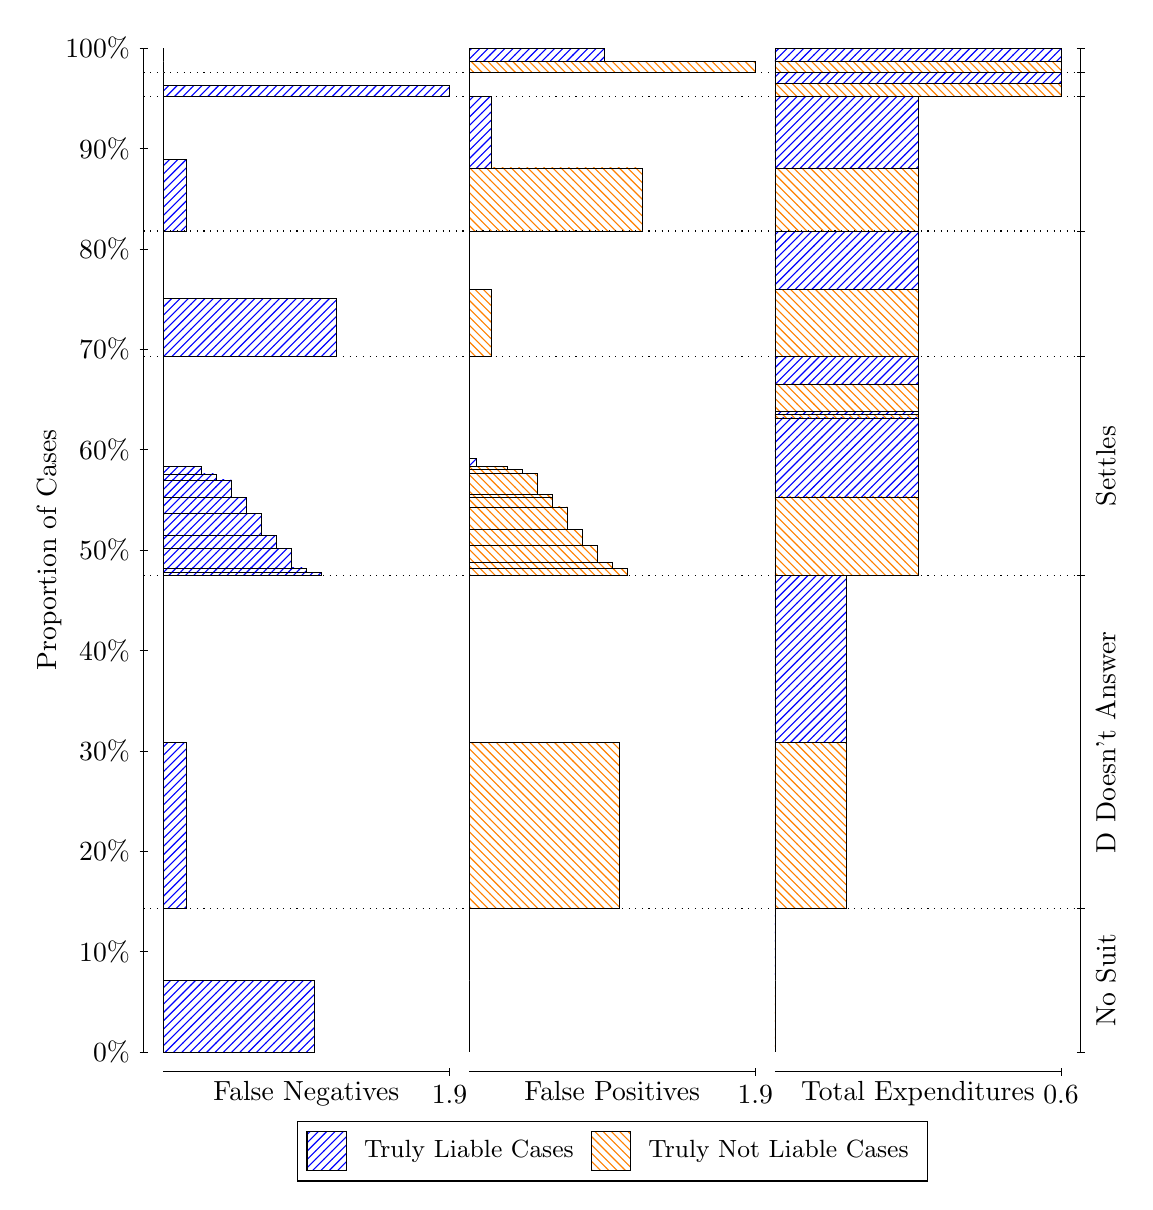
\begin{tikzpicture}
\draw[black, very thin] (1.5,1.75) -- (1.5,14.5);
\node[rotate=90, anchor=center] at (0.3, 8.125) {Proportion of Cases};
\draw[black, very thin] (1.45,1.75) -- (1.55,1.75);
\node[anchor=east] at (1.45, 1.75) {0\%};
\draw[black, very thin] (1.45,3.025) -- (1.55,3.025);
\node[anchor=east] at (1.45, 3.025) {10\%};
\draw[black, very thin] (1.45,4.3) -- (1.55,4.3);
\node[anchor=east] at (1.45, 4.3) {20\%};
\draw[black, very thin] (1.45,5.575) -- (1.55,5.575);
\node[anchor=east] at (1.45, 5.575) {30\%};
\draw[black, very thin] (1.45,6.85) -- (1.55,6.85);
\node[anchor=east] at (1.45, 6.85) {40\%};
\draw[black, very thin] (1.45,8.125) -- (1.55,8.125);
\node[anchor=east] at (1.45, 8.125) {50\%};
\draw[black, very thin] (1.45,9.4) -- (1.55,9.4);
\node[anchor=east] at (1.45, 9.4) {60\%};
\draw[black, very thin] (1.45,10.675) -- (1.55,10.675);
\node[anchor=east] at (1.45, 10.675) {70\%};
\draw[black, very thin] (1.45,11.95) -- (1.55,11.95);
\node[anchor=east] at (1.45, 11.95) {80\%};
\draw[black, very thin] (1.45,13.225) -- (1.55,13.225);
\node[anchor=east] at (1.45, 13.225) {90\%};
\draw[black, very thin] (1.45,14.5) -- (1.55,14.5);
\node[anchor=east] at (1.45, 14.5) {100\%};

\draw[black, very thin] (13.4,1.75) -- (13.4,14.5);
\draw[black, very thin] (13.35,1.75) -- (13.45,1.75);
\node[anchor=west] at (13.35, 1.75) {};
\draw[black, very thin] (13.35,3.5703) -- (13.45,3.5703);
\node[anchor=west] at (13.35, 3.5703) {};
\draw[black, very thin] (13.35,7.8) -- (13.45,7.8);
\node[anchor=west] at (13.35, 7.8) {};
\draw[black, very thin] (13.35,10.581) -- (13.45,10.581);
\node[anchor=west] at (13.35, 10.581) {};
\draw[black, very thin] (13.35,12.176) -- (13.45,12.176);
\node[anchor=west] at (13.35, 12.176) {};
\draw[black, very thin] (13.35,13.883) -- (13.45,13.883);
\node[anchor=west] at (13.35, 13.883) {};
\draw[black, very thin] (13.35,14.191) -- (13.45,14.191);
\node[anchor=west] at (13.35, 14.191) {};
\draw[black, very thin] (13.35,14.5) -- (13.45,14.5);
\node[anchor=west] at (13.35, 14.5) {};

\draw[black, very thin, pattern color=blue, pattern=north east lines] (1.75,1.75) rectangle (3.6623,2.6602);
\draw[black, very thin, pattern color=orange, pattern=north west lines] (1.75,2.6602) rectangle (1.75,3.5703);
\draw[black, very thin, pattern color=blue, pattern=north east lines] (1.75,3.5703) rectangle (2.0368,5.6852);
\draw[black, very thin, pattern color=orange, pattern=north west lines] (1.75,5.6852) rectangle (1.75,7.8);
\draw[black, very thin, pattern color=blue, pattern=north east lines] (1.75,7.8) rectangle (3.7579,7.8402);
\draw[black, very thin, pattern color=blue, pattern=north east lines] (1.75,7.8402) rectangle (3.5667,7.8981);
\draw[black, very thin, pattern color=blue, pattern=north east lines] (1.75,7.8981) rectangle (3.3754,8.149);
\draw[black, very thin, pattern color=blue, pattern=north east lines] (1.75,8.149) rectangle (3.1842,8.31);
\draw[black, very thin, pattern color=blue, pattern=north east lines] (1.75,8.31) rectangle (2.993,8.5881);
\draw[black, very thin, pattern color=blue, pattern=north east lines] (1.75,8.5881) rectangle (2.8018,8.7923);
\draw[black, very thin, pattern color=blue, pattern=north east lines] (1.75,8.7923) rectangle (2.6105,9.0147);
\draw[black, very thin, pattern color=blue, pattern=north east lines] (1.75,9.0147) rectangle (2.4193,9.0914);
\draw[black, very thin, pattern color=blue, pattern=north east lines] (1.75,9.0914) rectangle (2.2281,9.1893);
\draw[black, very thin, pattern color=orange, pattern=north west lines] (1.75,9.1893) rectangle (1.75,10.581);
\draw[black, very thin, pattern color=blue, pattern=north east lines] (1.75,10.581) rectangle (3.9491,11.322);
\draw[black, very thin, pattern color=orange, pattern=north west lines] (1.75,11.322) rectangle (1.75,12.176);
\draw[black, very thin, pattern color=blue, pattern=north east lines] (1.75,12.176) rectangle (2.0368,13.081);
\draw[black, very thin, pattern color=orange, pattern=north west lines] (1.75,13.081) rectangle (1.75,13.883);
\draw[black, very thin, pattern color=blue, pattern=north east lines] (1.75,13.883) rectangle (5.3833,14.027);
\draw[black, very thin, pattern color=orange, pattern=north west lines] (1.75,14.027) rectangle (1.75,14.191);
\draw[black, very thin, pattern color=orange, pattern=north west lines] (1.75,14.191) rectangle (1.75,14.33);
\draw[black, very thin, pattern color=blue, pattern=north east lines] (1.75,14.33) rectangle (1.75,14.5);
\draw[black, very thin, pattern color=orange, pattern=north west lines] (5.6333,1.75) rectangle (5.6333,2.6602);
\draw[black, very thin, pattern color=blue, pattern=north east lines] (5.6333,2.6602) rectangle (5.6333,3.5703);
\draw[black, very thin, pattern color=orange, pattern=north west lines] (5.6333,3.5703) rectangle (7.5456,5.6852);
\draw[black, very thin, pattern color=blue, pattern=north east lines] (5.6333,5.6852) rectangle (5.6333,7.8);
\draw[black, very thin, pattern color=orange, pattern=north west lines] (5.6333,7.8) rectangle (7.6412,7.8912);
\draw[black, very thin, pattern color=orange, pattern=north west lines] (5.6333,7.8912) rectangle (7.45,7.9659);
\draw[black, very thin, pattern color=orange, pattern=north west lines] (5.6333,7.9659) rectangle (7.2588,8.1807);
\draw[black, very thin, pattern color=orange, pattern=north west lines] (5.6333,8.1807) rectangle (7.0675,8.3885);
\draw[black, very thin, pattern color=orange, pattern=north west lines] (5.6333,8.3885) rectangle (6.8763,8.6714);
\draw[black, very thin, pattern color=orange, pattern=north west lines] (5.6333,8.6714) rectangle (6.6851,8.8007);
\draw[black, very thin, pattern color=orange, pattern=north west lines] (5.6333,8.8007) rectangle (6.6851,8.8347);
\draw[black, very thin, pattern color=orange, pattern=north west lines] (5.6333,8.8347) rectangle (6.4939,9.0941);
\draw[black, very thin, pattern color=orange, pattern=north west lines] (5.6333,9.0941) rectangle (6.3026,9.1496);
\draw[black, very thin, pattern color=orange, pattern=north west lines] (5.6333,9.1496) rectangle (6.1114,9.1917);
\draw[black, very thin, pattern color=blue, pattern=north east lines] (5.6333,9.1917) rectangle (5.7289,9.2895);
\draw[black, very thin, pattern color=blue, pattern=north east lines] (5.6333,9.2895) rectangle (5.6333,10.581);
\draw[black, very thin, pattern color=orange, pattern=north west lines] (5.6333,10.581) rectangle (5.9202,11.435);
\draw[black, very thin, pattern color=blue, pattern=north east lines] (5.6333,11.435) rectangle (5.6333,12.176);
\draw[black, very thin, pattern color=orange, pattern=north west lines] (5.6333,12.176) rectangle (7.8325,12.978);
\draw[black, very thin, pattern color=blue, pattern=north east lines] (5.6333,12.978) rectangle (5.9202,13.883);
\draw[black, very thin, pattern color=orange, pattern=north west lines] (5.6333,13.883) rectangle (5.6333,14.046);
\draw[black, very thin, pattern color=blue, pattern=north east lines] (5.6333,14.046) rectangle (5.6333,14.191);
\draw[black, very thin, pattern color=orange, pattern=north west lines] (5.6333,14.191) rectangle (9.2667,14.33);
\draw[black, very thin, pattern color=blue, pattern=north east lines] (5.6333,14.33) rectangle (7.3544,14.5);
\draw[black, very thin, pattern color=orange, pattern=north west lines] (9.5167,1.75) rectangle (9.5167,2.6602);
\draw[black, very thin, pattern color=blue, pattern=north east lines] (9.5167,2.6602) rectangle (9.5167,3.5703);
\draw[black, very thin, pattern color=orange, pattern=north west lines] (9.5167,3.5703) rectangle (10.425,5.6852);
\draw[black, very thin, pattern color=blue, pattern=north east lines] (9.5167,5.6852) rectangle (10.425,7.8);
\draw[black, very thin, pattern color=orange, pattern=north west lines] (9.5167,7.8) rectangle (11.333,8.8007);
\draw[black, very thin, pattern color=blue, pattern=north east lines] (9.5167,8.8007) rectangle (11.333,9.8039);
\draw[black, very thin, pattern color=orange, pattern=north west lines] (9.5167,9.8039) rectangle (11.333,9.8459);
\draw[black, very thin, pattern color=blue, pattern=north east lines] (9.5167,9.8459) rectangle (11.333,9.8861);
\draw[black, very thin, pattern color=orange, pattern=north west lines] (9.5167,9.8861) rectangle (11.333,10.235);
\draw[black, very thin, pattern color=blue, pattern=north east lines] (9.5167,10.235) rectangle (11.333,10.581);
\draw[black, very thin, pattern color=orange, pattern=north west lines] (9.5167,10.581) rectangle (11.333,11.435);
\draw[black, very thin, pattern color=blue, pattern=north east lines] (9.5167,11.435) rectangle (11.333,12.176);
\draw[black, very thin, pattern color=orange, pattern=north west lines] (9.5167,12.176) rectangle (11.333,12.978);
\draw[black, very thin, pattern color=blue, pattern=north east lines] (9.5167,12.978) rectangle (11.333,13.883);
\draw[black, very thin, pattern color=orange, pattern=north west lines] (9.5167,13.883) rectangle (13.15,14.046);
\draw[black, very thin, pattern color=blue, pattern=north east lines] (9.5167,14.046) rectangle (13.15,14.191);
\draw[black, very thin, pattern color=orange, pattern=north west lines] (9.5167,14.191) rectangle (13.15,14.33);
\draw[black, very thin, pattern color=blue, pattern=north east lines] (9.5167,14.33) rectangle (13.15,14.5);
\draw[black, dotted] (1.5,3.5703) -- (13.4,3.5703);
\draw[black, dotted] (1.5,7.8) -- (13.4,7.8);
\draw[black, dotted] (1.5,10.581) -- (13.4,10.581);
\draw[black, dotted] (1.5,12.176) -- (13.4,12.176);
\draw[black, dotted] (1.5,13.883) -- (13.4,13.883);
\draw[black, dotted] (1.5,14.191) -- (13.4,14.191);
\draw[black, very thin] (1.75,1.5) -- (5.3833,1.5);
\node[anchor=north] at (3.5667, 1.5) {False Negatives};
\draw[black, very thin] (5.3833,1.45) -- (5.3833,1.55);
\node[anchor=north] at (5.3833, 1.45) {1.9};

\draw[black, very thin] (5.6333,1.5) -- (9.2667,1.5);
\node[anchor=north] at (7.45, 1.5) {False Positives};
\draw[black, very thin] (9.2667,1.45) -- (9.2667,1.55);
\node[anchor=north] at (9.2667, 1.45) {1.9};

\draw[black, very thin] (9.5167,1.5) -- (13.15,1.5);
\node[anchor=north] at (11.333, 1.5) {Total Expenditures};
\draw[black, very thin] (13.15,1.45) -- (13.15,1.55);
\node[anchor=north] at (13.15, 1.45) {0.6};

\node[black, centered, rotate=90] at (13.72, 2.6602) {No Suit};
\node[black, centered, rotate=90] at (13.72, 5.6852) {D Doesn't Answer};
\node[black, centered, rotate=90] at (13.72, 9.1905) {Settles};





\draw (7.449999999999999,1.5) node[draw=none] (baseCoordinate) {};
\begin{scope}[align=center]
        \matrix[scale=0.5, draw=black, below=0.5cm of baseCoordinate, nodes={draw}, column sep=0.1cm]{
            \node[rectangle, draw, minimum width=0.5cm, minimum height=0.5cm, pattern=north east lines, pattern color=blue] {}; &
            \node[draw=none, font=\small] (B) {Truly Liable Cases}; &
            \node[rectangle, draw, minimum width=0.5cm, minimum height=0.5cm, pattern=north west lines, pattern color=orange] {}; &
            \node[draw=none, font=\small] (B) {Truly Not Liable Cases}; \\
            };
\end{scope}

\end{tikzpicture}
\end{document}